% Chapter 4
\chapter{Meta Heuristic Extended Local Planning}\label{ch:meta}

In this chapter we propose an approach to extend local planning systems, which are based on trajectory simulation and evaluation. The main idea is to apply well established Meta-Heuristic search algorithms to find good trajectories within a given sample of different applicable velocities, a robotic motion model and a given time period for simulation. 

We introduce trajectory selection extensions using a combination of meta-heuristic algorithms.

\begin{itemize}
\item{\bf{RST:}}    Random Restart method using simple term memory
\item{\bf{ILS-Tabu:}}  Based on Iterated Local Search and the use of a simple memory
\item{\bf{VNSB-Tabu:}} Based on Variable Neighborhood Search and the use of a simple memory and Best Improvement heuristic.
\item{\bf{VNSF-Tabu:}} Based on Variable Neighborhood Search and the use of a simple memory and Best Improvement heuristic.
\end{itemize}

The proposed methods are tested and refined and implemented into a robotic navigation system which already supports implementations of a local planner based on Dynamic Window Approach and Trajectory Rollout.

\begin{itemize}
\item{\bf{VNSB-POSNEG}} Refining VNSB-Tabu with short term memory
\item{\bf{VNSF-POSNEG}} Refining VNSF-Tabu with short term memory
\end{itemize}

The next section provides background information of meta-heuristic search, followed by a detailed description about the specific algorithms used for extending local planners.

The relevant local planners we took into consideration are the aforementioned Dynamic Window Approach and Trajectory Roll-out planner, which will be discussed at the end of this chapter.

\section{Meta-Heuristic Search}
The family of meta-heuristic algorithms is extremely successful in solving optimization problems, and are heavily used to solve hard problems whether they are  \emph{discrete} (Combinatorial Problems: e.g. Traveling Salesman Problem (TSP), MAX-Sat problem, Nurse Rostering problems (NRP), Classical Vehicle Routing Problem (CVRP)), or \emph{real-valued} (Continuous Optimization Problems: e.g. Pooling problem, Continues Min-Max problem).

In general an optimization problem and its solutions can be defined as follows (see \cite{blum2003metaheuristics}): 
\begin{definition}
An optimization problem $P = (S, f_c)$ can be defined by:\\
- a set of variables $X = \{x_1,\dots,x_n\} $;\\
- the values the variables can take (domains) $D_1,\dots,D_n$;\\
- constraints\\
- a cost function $f_c$ which has to be minimized, where $f_c:D_1 \times \dots \times D_n \rightarrow \mathbb{R}^+$; (which is the same as maximizing $-f_c$)\\
\end{definition}
The set of all possible assignments $S = \{s = \{(x_1,v_1),\dots,(x_n,v_n)\}\mid v_i \in D_i\}$ to the variables in $X$ is called the search or solution space.
A continues optimization problem is given if $S=\mathbb{R}^n$, otherwise if $S$ is discrete a discrete optimization problem is given.

Solutions which fulfill all constraints are called feasible solutions. 
It is not necessary to allow only feasible solutions in the search space, as accepting infeasible solutions during the search process can improve the overall solution quality and performance of the algorithm.

The solution $s^*\in S$ of an optimization problem with minimum cost is called a \emph{global} optimal solution. 
\begin{definition}
 A \emph{global} minimal solution is a solution $s^* \in S$ such that
 $f_c(s^*)\leq f_c(s) \forall s \in S$. 
\end{definition}
Since there might be more than one optimal solution $S^* \subseteq S$ is the set of \emph{globally} optimal solutions.

The main idea of meta-heuristic algorithms is to combine heuristic methods with strategic components which allow for an efficient and effective exploration of the search space. 

One basic heuristic approximation method is local search which given a initial solution tries to iteratively replace this solution with a better one in a defined neighborhood of the current solution. 
\begin{definition}
A neighborhood structure is a function $N:S\rightarrow 2^S$ that assigns to every $s \in S$ a set of neighbors $N(s) \subseteq S$. $N(s)$ is called the neighborhood of $s$.
\end{definition}
Defining the neighborhood function has an important influence on the good performance of many meta-heuristic algorithms. 
A neighborhood my be induced from metric functions introduced into $S$ given some notion of nearness within a given starting point. The process of a step from one local solution to another local solution is called a \emph{move}. Neighborhoods can also be induced by the set of applicable moves given a current solution (see \cite{gendreau2003tabusearch}).

Minimal solutions within a given neighborhood structure are defined as \emph{locally} minimal.
\begin{definition}
 A \emph{local} minimal solution w.r.t. a neighborhood structure $N$ is a solution $\hat{s}$  such that $\forall s_n \in N(\hat{s}):f_c(\hat{s})\leq f(s_n)$. 
\end{definition}
A visualization of the concepts of local vs. global minimal solutions is visualized in Figure~\ref{fig:fig_local_global}.
\begin{figure}[thpb]
   \footnotesize
   \centering
   \def\svgwidth{0.75\textwidth}
   \includesvg{figures/fig_local_global_minima}     
   \caption[]{This figures shows different kind of solutions to an optimization problem. The solutions $\hat{a}$ and $\hat{b}$ are local minimal solutions in the neighborhood $N_1(a)$ and $N_2(b)$ respectively, whereas the global minimal solution is $s^*$.}
   \label{fig:fig_local_global}
\end{figure}



\section{Single Solution Based Meta-Heuristics}
\subsection{Local Search}
The basic Local Search (LS) (cf. Algorithm~\ref{localsearchalgo}) finds a local optimum according to a cost function $cost(x)$ and a fixed sized region around an initial solution in the solution space. 
The set of solutions in this region is denoted as the neighborhood of $x$. The necessary steps to get from the initial solution to a solution in the neighborhood is called a move.

\begin{algorithm}
\caption{Local Search  (LS)}
\label{localsearchalgo}
\begin{algorithmic}[1] 
\State $x\gets$ initial solution
\Repeat
\State select a $x^\prime \in$ \Call{Neighborhood}{$x$}
\If {\Call{$cost$}{$x^\prime$} $\leq$ \Call{$cost$}{$x$}}
    \State $x\gets x^\prime$
\EndIf
\Until{stopping criteria satisfied}
\end{algorithmic}
\end{algorithm}

\subsection{Iterative Local Search}
A nice survey of Iterative Local Search including the basic algorithm (cf. Algorithm~\ref{ilsalgo}) can be found in \cite{lourencco2001iterated}. 
The main idea is to call a local search procedure iteratively, until a certain stopping criteria is satisfied. 
In each iteration the current solution might be perturbed by changing parts of the solution. 
The following local search takes this altered solution as a starting point and returns a new solution. 
If it satisfies an acceptance condition (e.g. the best solution so far), the process restarts with the new solution. 
In addition, a history of already found solutions may be used to steer perturbation and the acceptance test.
The steps of ILS are visualized in Figure~\ref{fig:fig_ils}

\begin{figure}[thb] 
   \footnotesize
   \centering
    \def\svgwidth{0.75\textwidth}
    \includesvg{figures/fig_ils}
    \caption[Pertubation step in ILS]{Pertubation of a local minimal solution $\hat{s}$, leads to an intermediate solution $s^\prime$. A local search is applied and a new local minimal solution $\hat{s}^\prime$ is found. (reproduced from \cite{blum2003metaheuristics})}  
     \label{fig:fig_ils}
\end{figure}
 
\begin{algorithm}
\caption{Iterative Local Search (ILS)}
\label{ilsalgo}
\begin{algorithmic}[1]
\State $x_0\gets$ initial solution
\State $x^*\gets$ \Call{LocalSearch}{$x_0$}
\Repeat
\State $x^\prime \gets$ \Call{Perturbation}{$x^{*}$,history}
\State $x^{*\prime} \gets$ \Call{LocalSearch}{$x^\prime$}
\State $x^* \gets$ \Call{AcceptanceCriterion}{$x^{*}$,$x^{*\prime}$,history}
\Until{stopping criteria satisfied}
\end{algorithmic}
\end{algorithm}

\subsection{Variable Neighborhood Search}
Instead of using a fixed neighborhood, the Basic Variable Neighborhood Search (cf. Algorithm~\ref{vnsalgo}) as presented in \cite{VNS} uses a neighborhood structure of possibly nested neighborhoods (cf. Equation~\ref{eq:nb}), which together are guaranteed to explore the whole solution space. 
\begin{equation}
N_k(x)=N_0(x),N_1(x),\dots,N_{k_{max}}(x)
\label{eq:nb}
\end{equation}
A specific neighborhood structure determines the topology of the search space within this neighborhood, or in other words a neighborhood specific landscape (see \cite{blum2003metaheuristics}).

Different neighborhood structures yield different landscapes. 
Furthermore a local minimal solution within one landscape, does not have to be a local minimal solution in another, and a search procedure will find a better local minimal solution (see Figure~\ref{fig:fig_vns}). 

\begin{figure}[thb]
   \footnotesize
   \centering
   \myfloatalign
   \captionsetup[subfigure]{labelformat=empty} 
    \subfloat[]
    {  
       \def\svgwidth{0.5\textwidth}
       \includesvg{figures/fig_vns_1}
    }
    \subfloat[]
    {  
       \def\svgwidth{0.5\textwidth}
       \includesvg{figures/fig_vns_2}
    }
    \caption[Search landscapes of two different neighborhoods.]{This figures shows two different landscape from different neighborhood structures. On the left image the local search stops at the local minimal solution $\hat{s}_1$. On the right the local search can proceed to a better local minimum $\hat{s}_2$. (reproduced from \cite{blum2003metaheuristics})}  
     \label{fig:fig_vns}
\end{figure}

In the shaking phase the algorithm chooses a random solution of the current neighborhood to avoid getting captured in local minima. 
If the solution found by the Local Search does not improve the next neighborhood will be considered (cf. Algorithm~\ref{changealgo}).

\begin{algorithm}
\caption{Variable Neighborhood Search (VNS)}
\label{vnsalgo}
\begin{algorithmic}[1]
\Function{VNS}{$x,k_{max}$}
\Repeat
\State $k \gets 1$
\Repeat
\State $x^{\prime} \gets$ \Call{Shake}{$x,k$}
\State $x^{\prime \prime}\gets$ \Call{LocalSearch}{$x^{\prime}$}
\State \Call{NeighborhoodChange}{$x,x^{\prime \prime},k$}
\Until{$k=k_{max}$}
\Until{stopping criteria satisfied}
\EndFunction
\end{algorithmic}
\end{algorithm}

\begin{algorithm}
\caption{Neighborhood Change}
\label{changealgo}
\begin{algorithmic}[1]
\Function{NeighborhoodChange}{$x,x^{\prime},k$}
\If {\Call{$cost$}{$x^\prime$} < \Call{$cost$}{$x$}}
    \State $x\gets x^\prime$
    \State $k\gets 1$
\Else
    \State $k\gets k+1$
\EndIf

\EndFunction
\end{algorithmic}
\end{algorithm}

\subsection{Tabu Search}
Another successful Meta-Heuristic strategy is Tabu Search (cf. Algorithm~\ref{tabualgo}) proposed in \cite{glover1999tabu}. 
To avoid local minima a Tabu list keeps track of moves which are not allowed during the exploration of the current neighborhood. 
In its simplest form the Tabu list includes all visited solutions. 
This might be too restrictive, or the list might grow too large, hence one can restrict the list to a certain length, and delete e.g. the oldest item in the list in each iteration. 
One advantage of this method is, that it can be easily combined with other Meta-Heuristic algorithms.

\begin{algorithm}
\caption{Tabu Search}
\label{tabualgo}
\begin{algorithmic}[1]
\State $Tabulist \gets 0$
\State $x\gets$ initial solution
\Repeat
 \State $X^\prime \gets$ \Call{Neighborhood}{$x$} $\not\in Tabulist$
 \State $x^\prime \gets$ best solution in $X^\prime$
 \State $Tabulist = Tabulist \cup \{x^\prime\}$
 \State $x \gets x^\prime$
 \If{$x$ is overall best solution}
   \State store $x$ as best solution
 \EndIf
\Until{stopping criteria satisfied}
\end{algorithmic}
\end{algorithm}

\section{Population Based Meta-Heuristics}
\subsection{Evolutionary Computation}
\subsection{Ant Colony Optimization}
\section{Classification and Comparison of Meta-Heuristics}

\section{Approach} \label{sec:Approach}
The aforementioned trajectory selection for forward movements, evaluation and collision test are costly operations. 
The focus lies on improving this part of the DWA algorithm. 
The trajectory sampling and selection of the DWA are implemented in python minimizing a simpler cost function $f_c(v,w)$ (cf. Equation~\ref{eq:simplecost}), where $f_g(v,w)$ is the distance of the center of the robot in the end position to a predefined goal position, and $f_o(v,w)$ is the maximal distance to an obstacle on the trajectory path.

\begin{equation}
   f_c(v,w)=\alpha f_g(v,w) - \beta f_o(v,w)
   \label{eq:simplecost}
\end{equation}

Instead of performing an exhaustive \textit{Brute Force} search on all velocity samples, Meta-Heuristic algorithms are here used to boost the search performance. 

The reduced search space are all tuples of forward and angular velocities $(v,w)$ within given limits $v_{min} \leq v \leq v_{max}$ and $w_{min} \leq w \leq w_{max}$ and a step size for discretization by fixing the number of samples.

\subsection{Neighborhood and Local Search (LS)}
The neighborhood of a solution is simply defined by making a number of discretization steps to reachable regions from the current solution velocity tuple. 
The 4-neighborhood makes a step by either increasing or decreasing the current linear and angular velocity by one discretization step (Manhattan distance $=1$). 
The 8-neighborhood takes all neighbors into account which are reachable in one discretization step (Moore neighborhood). 
16-neighborhood are all neighbors reachable in two steps. 
This process continues until the whole search space is the neighborhood. Figure~\ref{fig:fig_nb} visualizes the neighborhood structure.
\begin{figure}[thpb]
   \footnotesize
   \centering
   \def\svgwidth{\textwidth}
   \includesvg{figures/fig_neighborhood3d}     
   \caption[]{Neighborhood structure in the 2-dim velocity space.}
   \label{fig:fig_nb}
\end{figure}

Using Local Search the neighborhood is either exhaustively searched for the best solution (Best-Improvement heuristic) or stopped after finding the first improving solution (First-Improvement heuristic).

\subsection{Tabu List}
Instead of recording all steps made in a Local Search run, all visited states are marked as tabu and will not be considered as valid solution in future steps of the algorithm. 
The Tabu list is used by the other Meta-Heuristic algorithm during the Local Search.

\subsection{Iterated Local Search (ILS)}
The perturbation step is very simplified and just finds the next random valid velocity tuple. 
Instead of altering the current solution in each step, we make use of the history and apply it after a fixed amount of iterations. 
The algorithm can use a 4,8, and 16-neighborhood with Best Improvement heuristic for the Local Search.

\subsection{Variable Neighborhood Search (VNS)}
For the VNS algorithm local search is performed in one neighborhood until no improvement occurs. 
The shaking chooses a random solution in the current neighborhood. 
If the shaking does not yield any solution, because the whole neighborhood is tabu, or does not include a collision free trajectory, the next neighborhood is chosen. 
An ordering of neighborhoods according to their size yields the neighborhood structure $N_0(x)=$ 4-connected, $N_1(x)=$ 8-neighborhood, $\dots, N_k(x)=$ k-steps reachable neighborhood.
Larger neighborhoods are too costly to evaluate. 
Therefore the neighborhood structure is bounded above by $k_{max}=8$. 
If no improvement is made up to the $N_{k_{max}}$ neighborhood, a new initial solution is generated at random. 
The VNS algorithm can be used with Best-, or First-Improvement heuristic for the Local Search.

\section{Experiments}
To select a benchmark cost a brute force search is performed on random generated test instances, evaluating a fixed number of trajectories. 
The time the algorithm needs to find this benchmark solution is used to compare their performance.

All algorithm are tested using different minimal, and maximal velocities to account for different acceleration limits. 
The weighting coefficients of the cost function are fixed to $\alpha=0.01$ and $\beta=1$. The local goal is also at a fixed location in the map. 
The step size of the collision test is fixed to 0.015 meter. 
Forward simulation time is fixed to one second. 

The following 60 test instances include different obstacle counts and random placement of quadratic obstacles:
\begin{itemize}
\item 15 instances with 1 obstacle and side length 1 meter.
\item 15 instances with 3 obstacles and side length 1 meter.
\item 15 instances with 5 obstacles and side length 0.5 meter.
\item 15 instances with 25 obstacles and side length 0.1 meter.
\end{itemize}

Figure~\ref{fig:fig_instances} illustrates three random instances. 
A generated costmap together with a visualization of consecutive local path planning steps in a simulation is shown in Figure~\ref{fig:fig_instances_detail}.

%\begin{figure}[thpb]
\begin{figure}[thpb]
     \footnotesize
      \centering
      \myfloatalign
      \setlength\fboxsep{0pt}
      \setlength\fboxrule{0.5pt}
       \subfloat[]
       {  
           \fbox{
\includegraphics[width=0.3\textwidth]{figures/01_1_b_nocost.png}}
       } 
       \subfloat[]
       {  
           \fbox{
\includegraphics[width=0.3\textwidth]{figures/03_5_m_nocost.png}}
       } 
       \subfloat[]
       {  
           \fbox{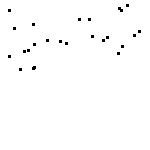
\includegraphics[width=0.3\textwidth]{figures/04_25_s_nocost.png}}
       }        
       \caption{Figures (a)-(c) show 3 out of 60 random instances for experiments. The instances differ in number and size of obstacles and are used for local costmap creation.}
      \label{fig:fig_instances}
   \end{figure}
   
\begin{figure}[thpb]
     \footnotesize
      \centering
      \setlength\fboxsep{0pt}
      \setlength\fboxrule{0.5pt}
       \def\svgwidth{\textwidth}
       %\fbox{\includesvg{figures/fig_inst_25_new}}
       \includesvg{figures/fig_inst_25_new}
		\caption[Local-path planning simulation.]{This figure shows three applications of the local planner in a simulated experiment. The greyscale background image visualizes obstacle costs of a generated costmap. Trajectories in green are drive-able, whereas red trajectories collide with obstacles. In each local planning step possible trajectories are weighted with respect to obstacle closeness and progression towards goal destination. For example in the second step a longer valid trajectory is rejected, while a shorter trajectory which stays farther away from obstacles is selected for execution. After three local planning applications the robot safely reaches the goal destination.}
		\label{fig:fig_instances_detail}
\end{figure}

The following list shows the tested algorithm:
\begin{itemize}
\item{\bf{Random Search with Tabu List:}} A repeated random guess of a velocity tuple $(v,w)$ (RST).
\item{\bf{Iterated Local Search:}} Performing Iterated Local Search with 4, 8 ,and 16 neighbors and Tabu List (ILS4, ILS8, ILS16).
\item{\bf{Variable Neighborhood Search:}} Variable Neighborhood search with Best-,and First-Improvement heuristic, and Tabu List (VNSB, VNSF).
\end{itemize}

\section{Test results}\label{sec:testresults}
All tests were performed on a 2.4 GHz, Intel Core 2 Duo processor using 4 GB RAM. 

In the first experiment the algorithms were applied to all 60 instances to evaluate a broad spectrum of possible environments. 
Figure~\ref{fig:fig_allworlds} illustrates the results using 240 trajectories, and using 2400 trajectory samples.
   \begin{figure}[thpb]
        \footnotesize
      \centering
      \def\svgwidth{0.7\textwidth}
      \includesvg{figures/fig_allworlds}
      \caption{This figure shows the results of testing all 60 randomly generated instances. The top figure shows the run time performance for 240 trajectories, and the bottom figure for 2400 trajectories. Compared to brute force search, the Meta-Heuristic algorithms show a significant improvement. }
      \label{fig:fig_allworlds}
   \end{figure}

 
The results show that all algorithms, including RST, outperform the Brute Force generate-and-test method significantly. 
As expected increasing the number of trajectories greatly favors the Meta-Heuristic algorithms, since they benefit from larger search spaces. 
Notice that ILS and VNS algorithms differ apparently from the RST by exhibiting much smaller variance in their test results, indicating that randomization alone is not enough to achieve very good and stable performance.
Furthermore the VNS exhibit a more stable performance than the ILS methods. 
Comparing the ILS algorithms reveals the connection of the search space size to the size of the neighborhood. 
A small number of trajectories benefits smaller sized neighborhoods, whereas increasing the number of trajectories benefits larger neighborhoods. 

The following tests only include the VNSF, VNSB and ILS4 algorithms. 
The algorithms are executed with specific world instances, and repeated 50 times. 
The results in Figure~\ref{fig:fig_special} show again that the VNS algorithms significantly outperform the Brute Force method. 

\begin{figure}[thb]
   \myfloatalign
   %\captionsetup[subfigure]{labelformat=empty} 
    \subfloat[]
    {  
       \def\svgwidth{\textwidth}
       \includesvg{figures/fig_6_40}
    }\\
    \subfloat[]
    {  
       \def\svgwidth{\textwidth}
       \includesvg{figures/fig_12_80}
    }
    \caption[Experiment: Trajectory size comparison]{The results of 50 consecutively executions with (a) 240 and (b) 960 trajectories, on particular instances which differ in number and size of obstacles. The blue line marks the run time for brute force search, which is used as a benchmark.}  
     \label{fig:fig_special}
\end{figure}
   
Analyzing the results of the ILS4 algorithms shows that a too small environment will quickly degrade to random search. 
Here the use of a neighborhood structure pays off and the VNS approaches perform evidently better than ILS. 
In addition, the results show that the algorithms perform good independent of number and size of obstacles.

As for nearly all optimization problems, the No Free Lunch theorems \cite{wolpert1997no} apply to the local planning domain. 
Looking at all the results, there is no clear winner among the algorithms. 
Nevertheless using Variable Neighborhood search with Tabu List and Best Improvement heuristic seem to yields the best and most stable overall performance. 

In general the run time of the python implementation is not very efficient compared to tuned C++ implementations. 
Therefore the absolute numbers of the run time evaluations should be handled with care. 
